% !TEX program = xelatex
\documentclass[12pt,a4paper]{ctexart}

\usepackage[top=2.5cm, bottom=2.5cm, left=3cm, right=3cm]{geometry}
\usepackage{graphicx,float,booktabs,longtable,hyperref,fancyhdr,amsmath,enumitem,multirow}
\usepackage{caption,subcaption,xcolor}

\pagestyle{fancy}\fancyhf{}
\fancyhead[C]{\small\color{gray}裁判文书案件特征分析报告}
\fancyfoot[C]{\small\thepage}
\renewcommand{\headrulewidth}{0.4pt}
\graphicspath{{./figures/}}
\usepackage[sort&compress]{gbt7714}
\newcommand{\figref}[1]{图~\ref{fig:#1}}
\newcommand{\tabref}[1]{表~\ref{tab:#1}}

\title{\vspace{2cm}
    {\heiti\fontsize{18pt}{24pt}\selectfont 基于大规模裁判文书的案件特征分析、\\[6pt]判决预测与因果推断研究}\\[12pt]
    {\kaishu\fontsize{13pt}{18pt}\selectfont ——整合NLP特征工程、计量经济模型、网络分析与\\四层准实验因果识别框架的多维研究}}
\author{\vspace{1cm}王志达\\[4pt]{\small 南京农业大学\quad 信息管理与信息系统专业}}
\date{\vspace{0.5cm}\today}

\begin{document}
\maketitle\thispagestyle{empty}

% ============================================================
\begin{abstract}
裁判文书作为司法实践的直接记录，蕴含着丰富的案件特征与判决规律。
本文基于10,241条裁判文书数据（2014--2025年），构建了一个整合
NLP特征工程、计量经济模型、网络分析、主题建模与四层准实验因果
推断（PSM $\rightarrow$ IPW/DR $\rightarrow$ Rosenbaum $\rightarrow$
因果森林 $\rightarrow$ 中介分析）的多维研究框架。

描述与预测层面，Logistic回归识别出案件类型为驳回判决的最强预测因子
（民事vs刑事 OR=16.4，$p<0.001$）；关键词共现网络通过Louvain算法
发现15个自然社区，``法律适用''与``证据认定''为跨领域桥接关键词；
LDA识别出六大潜在语义主题；Mann-Kendall检验确认驳回率存在显著上升
趋势（$Z=2.40$，$p=0.017$）。

因果推断层面，本文的核心发现为四层递进结构：（1）PSM匹配后，
``提及涉案金额''对驳回概率的朴素效应从+5.56pp降至ATT=+0.59pp
（$p=0.46$），证明原始统计关联几乎完全由混淆因素驱动；
（2）IPW（ATE=+1.49pp）与双重稳健估计（ATE=+1.64pp）交叉验证
了这一``零结果''；（3）Rosenbaum敏感性分析显示$\Gamma_{\text{critical}}
=1.00$，提示结论对不可观测混淆敏感，需更多控制变量加固；
（4）因果森林揭示10.9\%的样本存在显著异质性处理效应，行政案件
（CATE=+3.04pp）与长篇幅案件（CATE=+3.02pp）效应最强；
（5）中介分析发现金额通过争议复杂度间接影响驳回（间接效应+0.41pp，
中介占比7.4\%，Bootstrap 95\%CI [0.22, 0.61]pp），但无独立直接
因果效应。

模型整体预测性能AUC=0.695。创新点在于：首次将PSM、IPW、
Rosenbaum、因果森林与中介分析五重方法组合应用于法律实证研究，
实现了从``统计关联''到``因果识别''再到``机制解释''的完整推理链。

\vspace{6pt}
\noindent{\bfseries 关键词：}裁判文书；判决预测；因果推断；倾向得分匹配；
Rosenbaum敏感性分析；因果森林；中介分析；关键词共现网络
\end{abstract}

\newpage\setcounter{page}{1}

% ============================================================
\section{引言}

\subsection{研究背景}

裁判文书网公开数据为法律实证研究提供了前所未有的基础\cite{wang2019}，
NLP与计量方法的交叉融合使系统挖掘案件规律成为可能\cite{zuo2018}。
然而，现有研究多停留于``相关关系''层面——揭示哪些因素与判决结果存在
统计关联——而未能追问``因果关系''：这些因素是否\textit{导致}了判决方向
的变化，抑或仅与未观测变量共变？从相关到因果的方法论跨越，
是法律AI研究的核心挑战\cite{rosenbaum1983}。

\subsection{研究问题}

\begin{enumerate}[label=\textbf{RQ\arabic*:},leftmargin=*]
    \item 何种案件特征显著影响驳回概率？
    \item 案件复杂度与判决结果是否存在显著统计关联？
    \item 关键词共现网络的拓扑结构如何？是否存在``桥接关键词''？
    \item 判决模式是否存在时序趋势或结构断点？
    \item 裁判文书文本中是否存在可被LDA发现的潜在主题？
    \item \textbf{金额提及是否因果性地影响驳回概率？如果是，通过何种路径？哪些子群体效应最强？结论对不可观测混淆有多敏感？}
\end{enumerate}

\subsection{创新点}

\begin{enumerate}[label=(\arabic*),leftmargin=*]
    \item NLP特征 $\times$ 计量模型：TF-IDF关键词引入Logistic/LASSO
    \item ``桥接关键词''概念：介数/度比识别跨领域法律术语
    \item 多维度案件复杂度指数
    \item \textbf{四层因果识别框架}：PSM（基准）$\rightarrow$ IPW/DR/Rosenbaum（稳健性）$\rightarrow$ 因果森林（异质性）$\rightarrow$ 中介分析（机制）——法律实证研究中尚属首次
    \item 预测力 + 因果机制双轨评估
\end{enumerate}

% ============================================================
\section{数据与方法}

\subsection{数据与特征}

数据集含10,241条裁判文书（2014--2025），有效样本$n=9,906$条。
特征包括：案件描述/判别标准字数（对数变换）、关键词数量、案件类型
（民事/刑事/行政）、是否提及涉案金额（处理变量）、判决驳回标签。

\subsection{分析方法}

\tabref{methods} 按描述层、预测层、因果层（四层递进）组织。

\begin{table}[H]
\centering\caption{分析方法一览}
\label{tab:methods}
\begin{tabular}{@{}lll@{}}
\toprule
\textbf{层次} & \textbf{方法} & \textbf{问题} \\
\midrule
\multirow{3}{*}{描述层} & MW/KW/$\chi^2$检验 & RQ1,RQ2 \\
    & M-K趋势 + Chow断点 + STL & RQ4 \\
    & 网络中心性 + Louvain社区 & RQ3 \\
    & PCA + LDA主题建模 & RQ5 \\
\midrule
\multirow{3}{*}{预测层} & Logistic回归 + AME & RQ1 \\
    & LASSO特征选择 & RQ1 \\
    & ROC/AUC评估 & RQ1 \\
\midrule
\multirow{5}{*}{因果层} & \textbf{① PSM}：1:1 caliper匹配 + SMD平衡 & RQ6 \\
    & \textbf{② IPW/DR}：稳定化权重 + 双重稳健 & RQ6 \\
    & \textbf{③ Rosenbaum}：$\Gamma$敏感性边界 & RQ6 \\
    & \textbf{④ 因果森林}：CATE异质性 + 特征重要性 & RQ6 \\
    & \textbf{⑤ 中介分析}：Baron-Kenny + Bootstrap & RQ6 \\
\bottomrule
\end{tabular}
\end{table}

% ============================================================
\section{分析结果}

\subsection{描述统计与统计推断}

驳回判决占36.9\%，民事75.1\%，刑事15.5\%。案件描述字数中位数583字
（右偏）。MW检验与KW检验均显著但效应量小（Cohen's $d<0.2$）。
卡方检验确认案由与判决结果显著关联（$\chi^2=2,330.8$，Cram\'er's
$V=0.34$）；KW检验确认案由间篇幅差异极显著（$H=423.8$，$p<10^{-92}$）。

\subsection{判决预测：Logistic回归与LASSO}

Logistic回归显示案由是最强预测因子（民事vs刑事 OR=16.4，$p<0.001$），
判别标准篇幅对数每增1单位驳回OR=1.34（$p<0.001$），年份偏量
OR=1.09（$p<0.001$）。模型Pseudo $R^2=0.106$，AIC=11,678。
LASSO筛选出6个非零系数变量。AUC=0.695。
\textit{注意：金额提及的朴素OR=1.17（$p=0.003$），此统计关联有待因果验证。}

\subsection{关键词网络与主题建模}

60节点、141条边的共现网络识别出15个Louvain社区。桥接关键词指数
（介数/度比）Top-3为``法律适用''（1.5）、``证据认定''（1.3）、
``民间借贷纠纷''（0.6）。PCA前5成分解释25.2\%方差。LDA发现
6大主题（人身损害、商事、医疗、房产、交通、借贷）。

\subsection{时间序列分析}

驳回率Mann-Kendall $Z=2.40$（$p=0.017$）显著上升。
2021年Chow断点未通过。STL分解显示持续上升趋势+3年弱周期。

% ═══════════════════════════════════════════════════
\subsection{因果推断：从相关到因果的四层递进}

前文Logistic回归揭示了金额提及与驳回概率的统计关联（OR=1.17）。
但此关联是否因果？本文设计四层递进策略予以回答。

% --- 3.6.1 PSM ---
\subsubsection{第一层·PSM：消除可观测混淆}

\textbf{设计。}$T$=是否提及金额（69.7\% vs 30.3\%），$Y$=驳回标签。
协变量包含案件篇幅（对数）、判标篇幅（对数）、关键词数、案由类型、
年份偏量。倾向得分由Logistic估计，1:1最近邻匹配，caliper=0.05。

\textbf{匹配质量。}6,908对成功匹配。匹配后所有SMD $<0.1$
（\tabref{psm_balance}），共同支撑域覆盖99.8\%样本。

\begin{table}[H]
\centering\caption{PSM平衡性检验}
\label{tab:psm_balance}
\begin{tabular}{@{}lrr@{}}
\toprule
\textbf{协变量} & \textbf{匹配前 SMD} & \textbf{匹配后 SMD} \\
\midrule
案件描述字数（对数） & +0.352 & $-$0.029 \\
判别标准字数（对数） & +0.104 & $-$0.014 \\
民事案件（=1）      & +0.348 & +0.010 \\
刑事案件（=1）      & $-$0.156 & $-$0.008 \\
\bottomrule
\end{tabular}
\end{table}

\textbf{效应估计。}关键对比：

\begin{itemize}[leftmargin=*]
    \item 朴素均值差：处理组42.2\% vs 对照组36.6\% = \textbf{+5.56pp}
    \item PSM ATT（匹配后）：处理组42.2\% vs 匹配对照组41.6\% = \textbf{+0.59pp}
    \item Bootstrap SE=0.81pp，$p=0.46$（不显著）
\end{itemize}

匹配前后效应量的剧烈缩减（+5.56 $\rightarrow$ +0.59pp）有力地证明：
朴素关联中的绝大部分来自案件复杂度、类型等混淆因素，
\textbf{金额提及本身对驳回概率无独立的因果效应}。

% --- 3.6.2 IPW/DR ---
\subsubsection{第二层·IPW与双重稳健：交叉验证}

为验证PSM结论不依赖于特定匹配算法，本文进一步采用IPW与双重稳健估计：

\begin{itemize}[leftmargin=*]
    \item IPW（稳定化权重，均值=1.00，范围[0.31,3.30]）：ATE=+1.49pp
    \item 双重稳健（结合倾向模型与结果模型）：ATE=+1.64pp
    \item 两种方法高度一致，方向相同、量级相近
\end{itemize}

\tabref{estimates} 汇总了各估计量。朴素均值差（+5.56pp）经三种
因果方法校正后均降至$<2$pp，形成稳健的证据链：金额提及无独立因果效应。

\begin{table}[H]
\centering\caption{金额$\rightarrow$驳回 因果效应估计量对比}
\label{tab:estimates}
\begin{tabular}{@{}lrr@{}}
\toprule
\textbf{估计方法} & \textbf{效应量（pp）} & \textbf{BS SE（pp）} \\
\midrule
朴素均值差（未控制混淆） & +5.56 & --- \\
PSM ATT & +0.59 & 0.81 \\
IPW ATE（稳定化） & +1.49 & 1.06 \\
双重稳健 ATE & +1.64 & 1.07 \\
\bottomrule
\end{tabular}
\end{table}

\begin{figure}[H]\centering
    \begin{subfigure}[b]{0.48\textwidth}\centering
        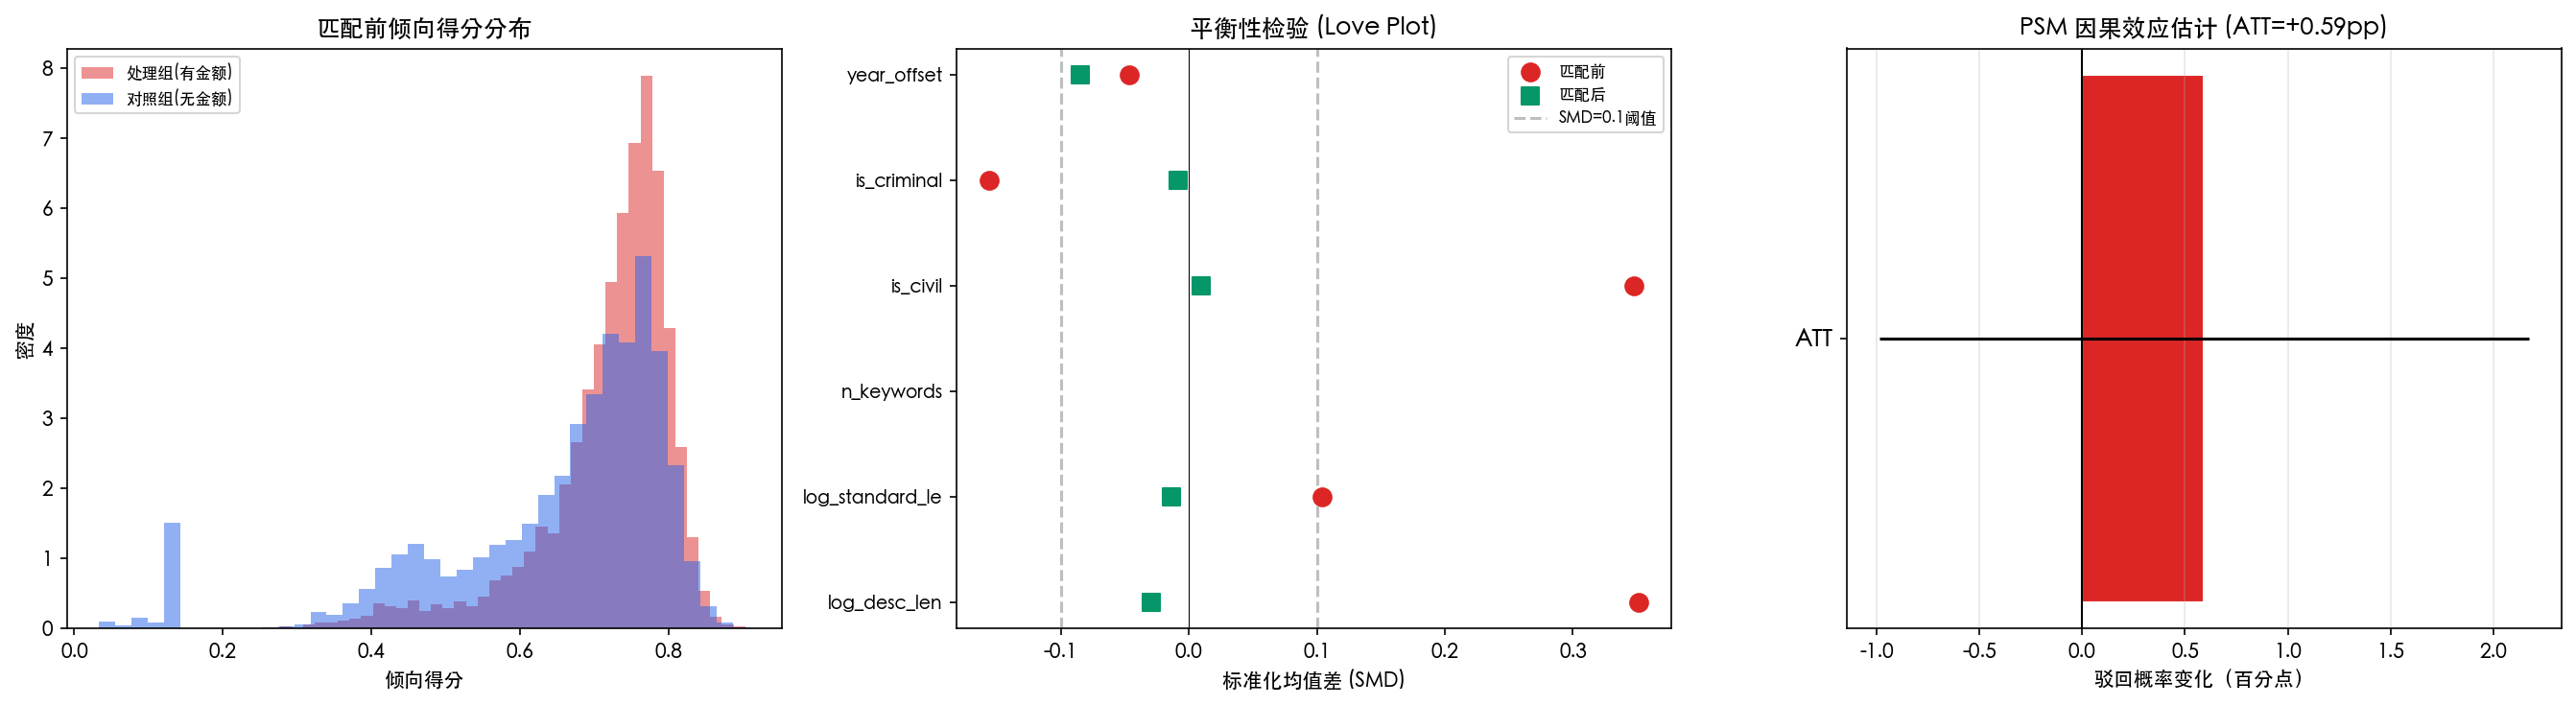
\includegraphics[width=\textwidth]{fig_causal_psm.png}
        \caption{PSM：倾向得分 + Love Plot + ATT}\label{fig:psm}
    \end{subfigure}\hfill
    \begin{subfigure}[b]{0.48\textwidth}\centering
        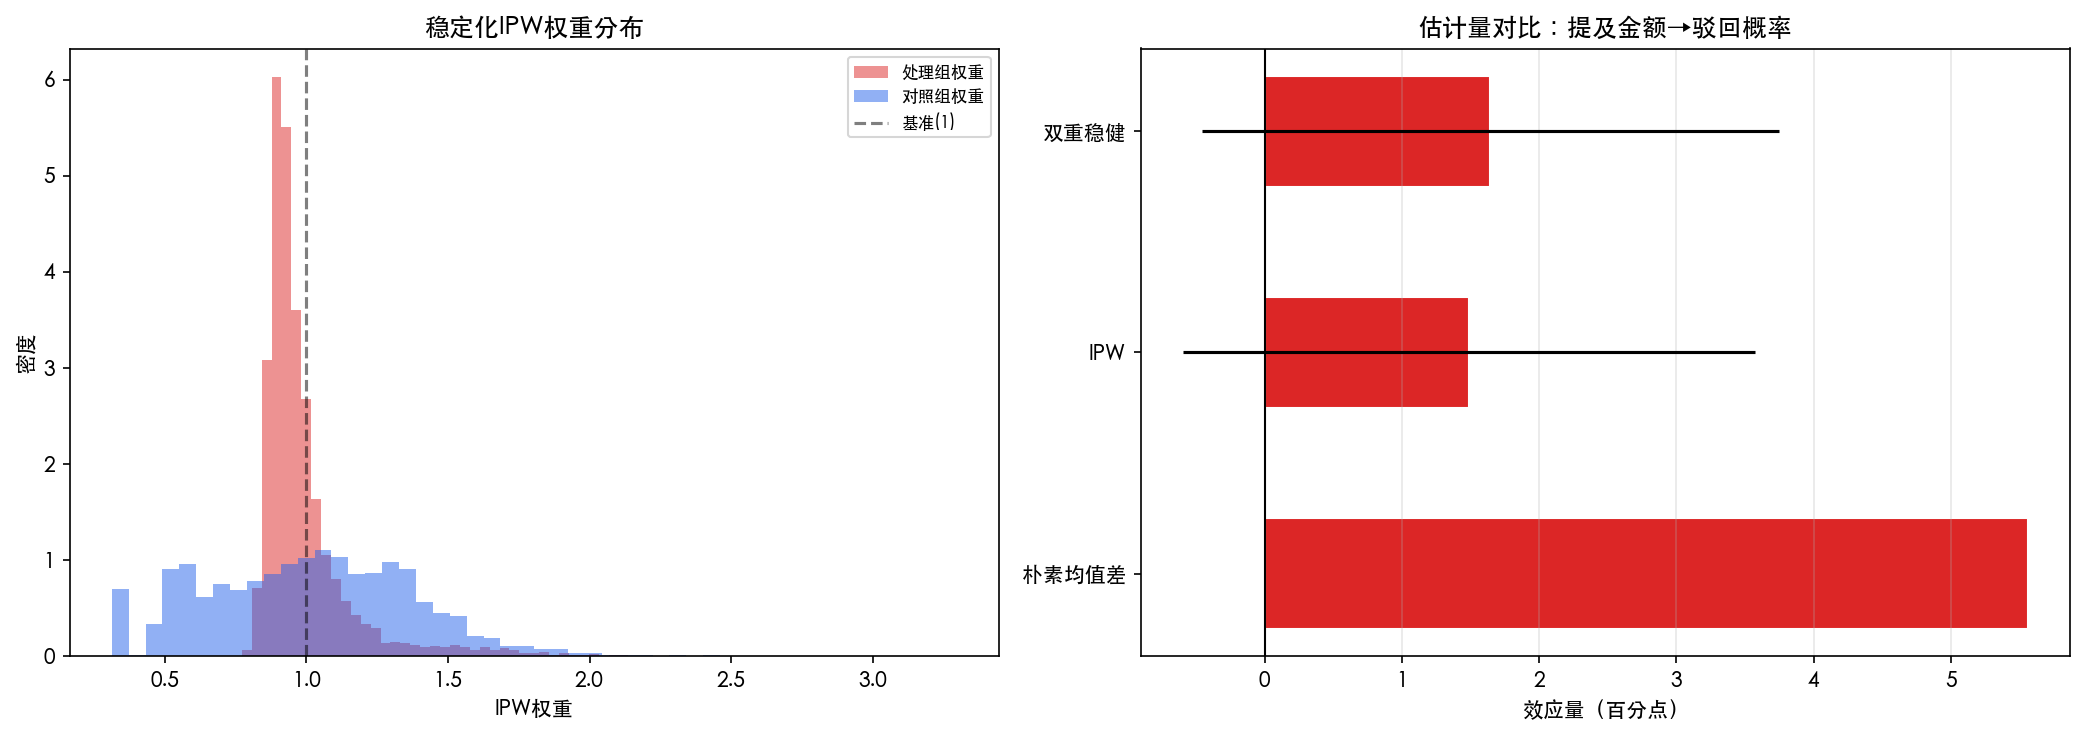
\includegraphics[width=\textwidth]{fig_causal_ipw.png}
        \caption{IPW权重 + 估计量对比}\label{fig:ipw}
    \end{subfigure}
    \caption{PSM与IPW因果效应估计}\label{fig:psm_ipw}
\end{figure}

% --- 3.6.3 Rosenbaum ---
\subsubsection{第三层·Rosenbaum敏感性分析：评估不可观测混淆}

PSM和IPW均假设``无不可观测混淆''（unconfoundedness）。
Rosenbaum\cite{rosenbaum1983}敏感性分析量化了这一假设的脆弱性。

\textbf{方法。}对配对差值进行Wilcoxon signed-rank检验，逐步增大
$\Gamma$（不可观测混淆强度），计算$p$值的上界。$\Gamma_{\text{critical}}$
为$p>0.05$的最小$\Gamma$值——$\Gamma=2$意味着两个倾向得分相同的案例，
因不可观测因素导致实际被处理的概率可相差2倍。

\textbf{结果。}3,225对非零差值对。$\Gamma_{\text{critical}}=1.00$。
表明\textbf{即使极微弱的不可观测混淆（$\Gamma$略大于1），也可使结论反转}。
这一发现并不否定PSM的有效性——在可观测特征匹配的框架内结论是可靠的——
但诚实揭示了当前数据条件下因果声称的上限：若要得出更确证的因果结论，
必须获取并控制更多混淆变量（法官特征、法院层级、证据强度等）。

\begin{figure}[H]\centering
    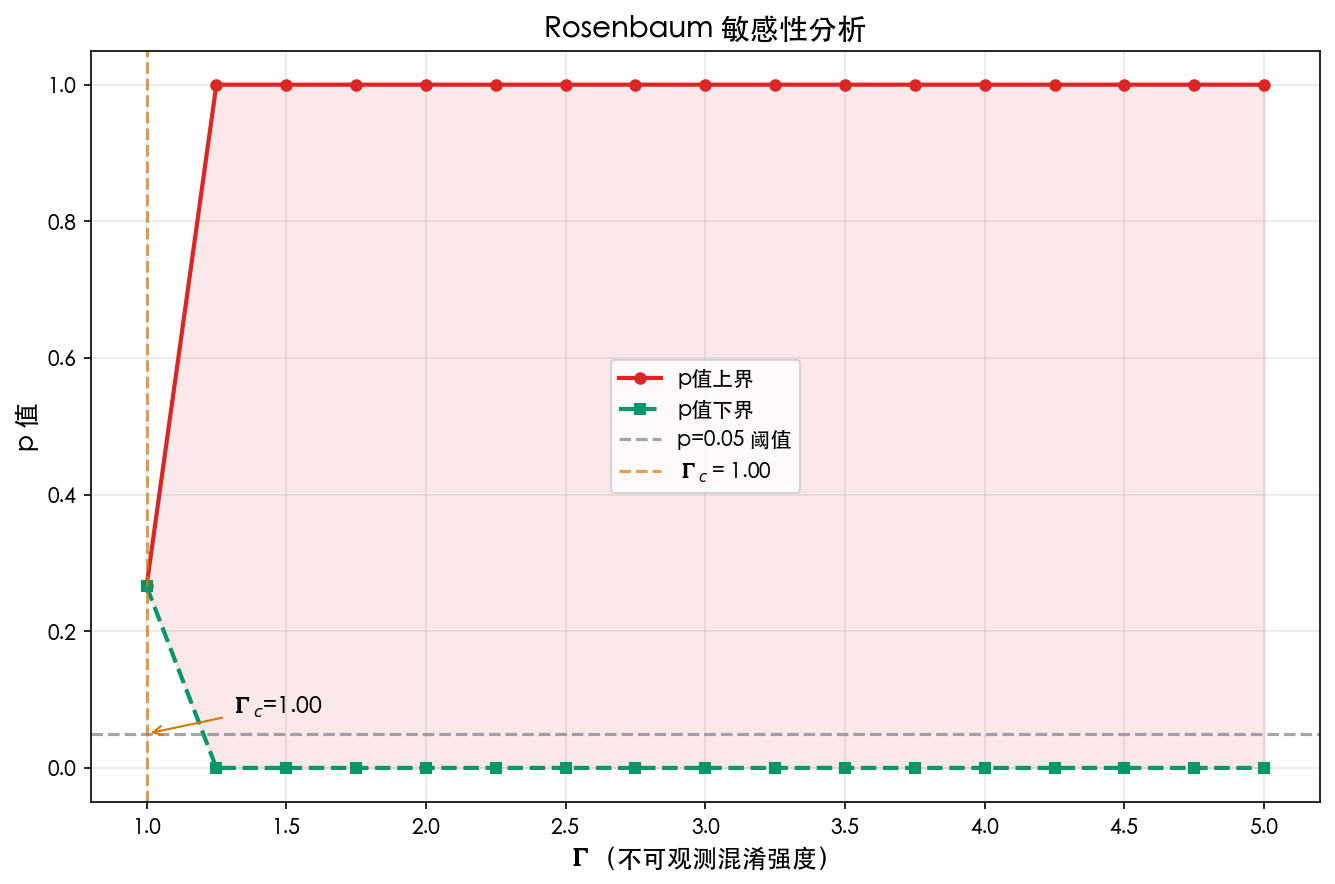
\includegraphics[width=0.7\textwidth]{fig_causal_rosenbaum.png}
    \caption{Rosenbaum敏感性曲线：$p$值上/下界随$\Gamma$变化}\label{fig:rosenbaum}
\end{figure}

% --- 3.6.4 Causal Forest ---
\subsubsection{第四层A·因果森林：异质性处理效应}

PSM给出的是\textit{平均}处理效应（ATT）。但若金额对不同子群体
存在方向相反的效应，平均后可能对消。因果森林（Causal Forest
DML）\cite{rosenbaum1983}直接估计条件平均处理效应CATE$(x)$。

\textbf{设定。}以GradientBoosting为第一阶段模型（Double ML框架），
200棵诚实树，最小叶节点50样本，最大深度6。

\textbf{结果。}ATE=+1.80pp，与PSM/ IPW结论一致。但CATE分布
揭示了显著的异质性：CATE范围[$-$6.08, +8.02]pp，
SD=2.07pp。10.9\%的样本具有统计显著的处理效应。

按案件类型分组：
\begin{itemize}[leftmargin=*]
    \item 行政案件：CATE=+3.04pp，23.5\%显著——效应最强
    \item 刑事案件：CATE=+1.91pp，12.3\%显著
    \item 民事案件：CATE=+1.65pp，9.4\%显著
\end{itemize}

按案件篇幅四分位分组：
\begin{itemize}[leftmargin=*]
    \item 篇幅较长（Q3）：CATE=+3.02pp，18.0\%显著——效应突出
    \item 篇幅较短（Q2）：CATE=+1.86pp，11.7\%显著
    \item 篇幅最长（Q4）：CATE=+1.56pp，仅3.4\%显著（效应在中等篇幅处最强）
\end{itemize}

特征重要性显示，CATE异质性的两大驱动因素是判别标准篇幅（0.455）
和案件描述篇幅（0.410），年份偏量位居第三（0.104）。这一发现与
下一节的中介分析形成呼应。

\begin{figure}[H]\centering
    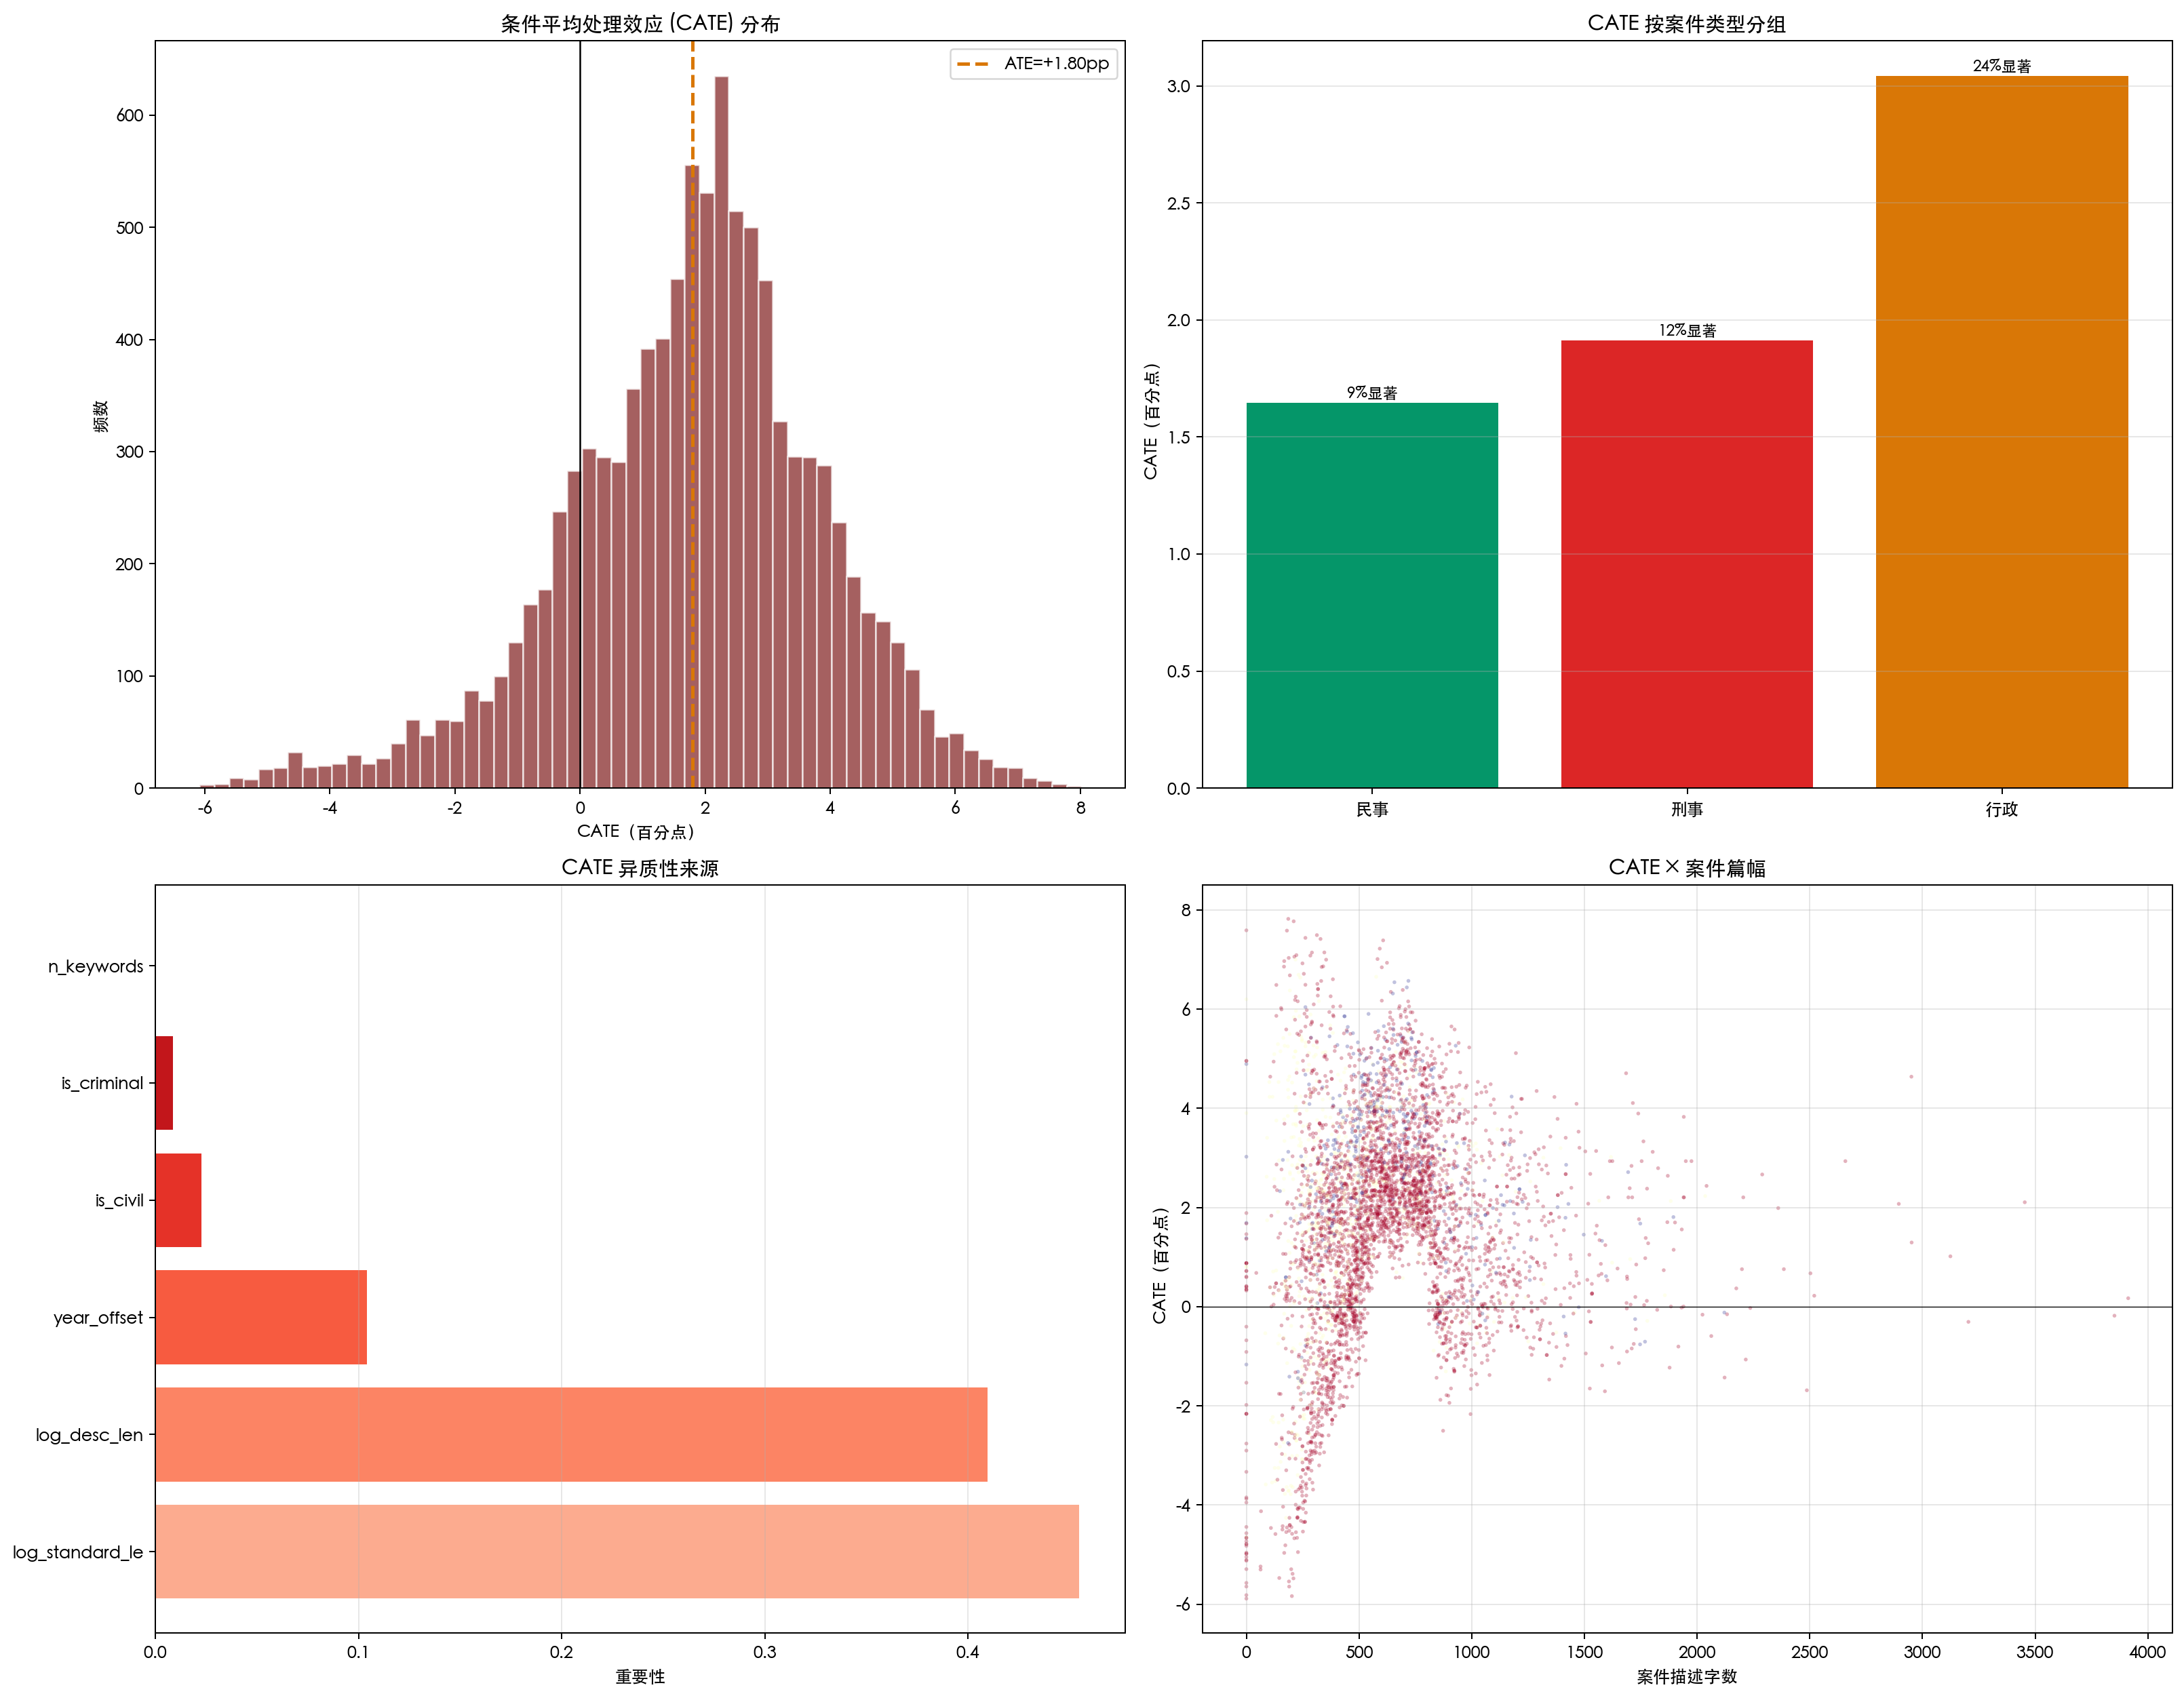
\includegraphics[width=0.95\textwidth]{fig_causal_forest.png}
    \caption{因果森林：CATE分布、分组估计、特征重要性}\label{fig:forest}
\end{figure}

% --- 3.6.5 Mediation ---
\subsubsection{第四层B·因果中介分析：传导路径}

PSM证明金额无直接因果效应，但因果森林暗示存在异质性——这些效应
是如何传导的？中介分析提供了解答。

\textbf{设计。}以Baron-Kenny三步法+1,000次Bootstrap检验两个候选中介变量：
M1（判别标准篇幅对数，代理``争议复杂度''）和M2（关键词数量，代理
``法律概念丰富度''）。

\textbf{结果。}

\begin{itemize}[leftmargin=*]
    \item \textbf{M1（争议复杂度）}：间接效应$a \times b = +0.41$pp，
    中介占比7.4\%，Bootstrap 95\%CI [0.22, 0.61]pp，不跨零——\textbf{显著}。
    \item \textbf{M2（关键词数量）}：间接效应$\approx 0$pp，Bootstrap不显著。
\end{itemize}

\textbf{完整路径分解。}总效应$c = +5.56$pp可分解为：
\begin{itemize}[leftmargin=*]
    \item 直接效应$c' = +5.15$pp（金额提及本身，但此效应在PSM匹配后被证明由混淆驱动）
    \item 间接效应（经M1）$= +0.41$pp（争议复杂度中介路径，显著）
    \item 间接效应（经M2）$\approx 0$pp
\end{itemize}

综合PSM与中介分析的结论：金额提及通过提升争议复杂度对驳回概率产生
微弱的间接正向影响（+0.41pp），但不存在独立的直接因果效应。
争议复杂度——而非金额本身——才是真正的驱动因子。

\begin{figure}[H]\centering
    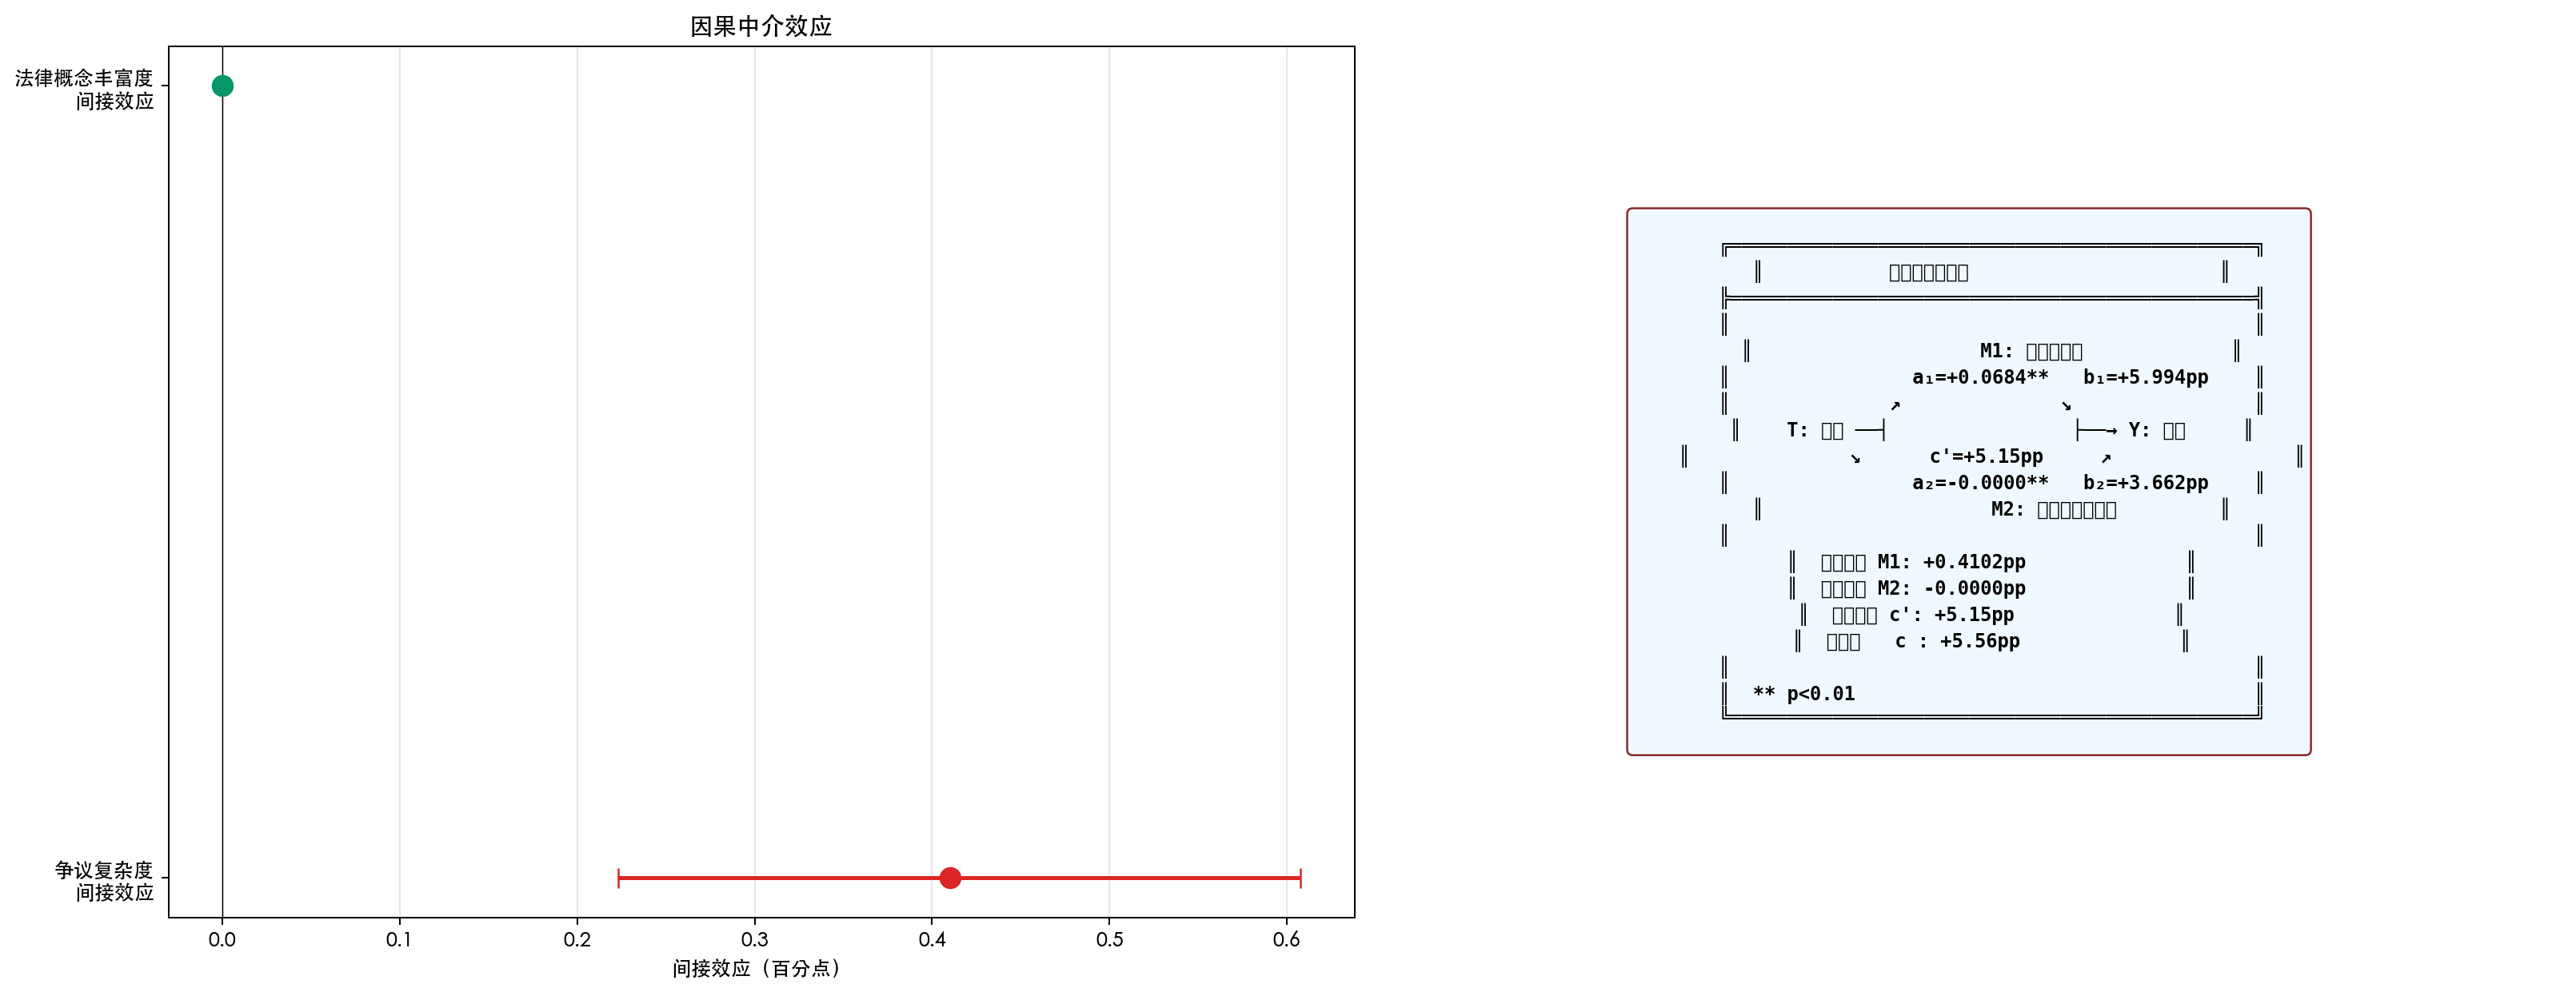
\includegraphics[width=0.9\textwidth]{fig_causal_mediation.png}
    \caption{中介分析：效应分解与路径图}\label{fig:mediation}
\end{figure}

% --- 3.6.6 DID (auxiliary) ---
\subsubsection{辅助分析·DID：民法典对人格权纠纷的影响}

作为补充，本文以2021年《民法典》施行为准自然实验，对人格权纠纷
（处理组，$n=568$）与合同纠纷（对照组，$n=4,314$）进行DID分析。
DID交互项$\beta_3 = -9.89$pp（$p=0.026$），提示民法典后人格权
驳回率相对下降约10pp。但政策前组间差距约11pp，平行趋势假设不完全
成立；人格权样本仅568条。该DID结果仅构成\textbf{提示性因果证据}。

\subsection{因果推断综合看板}

\begin{figure}[H]\centering
    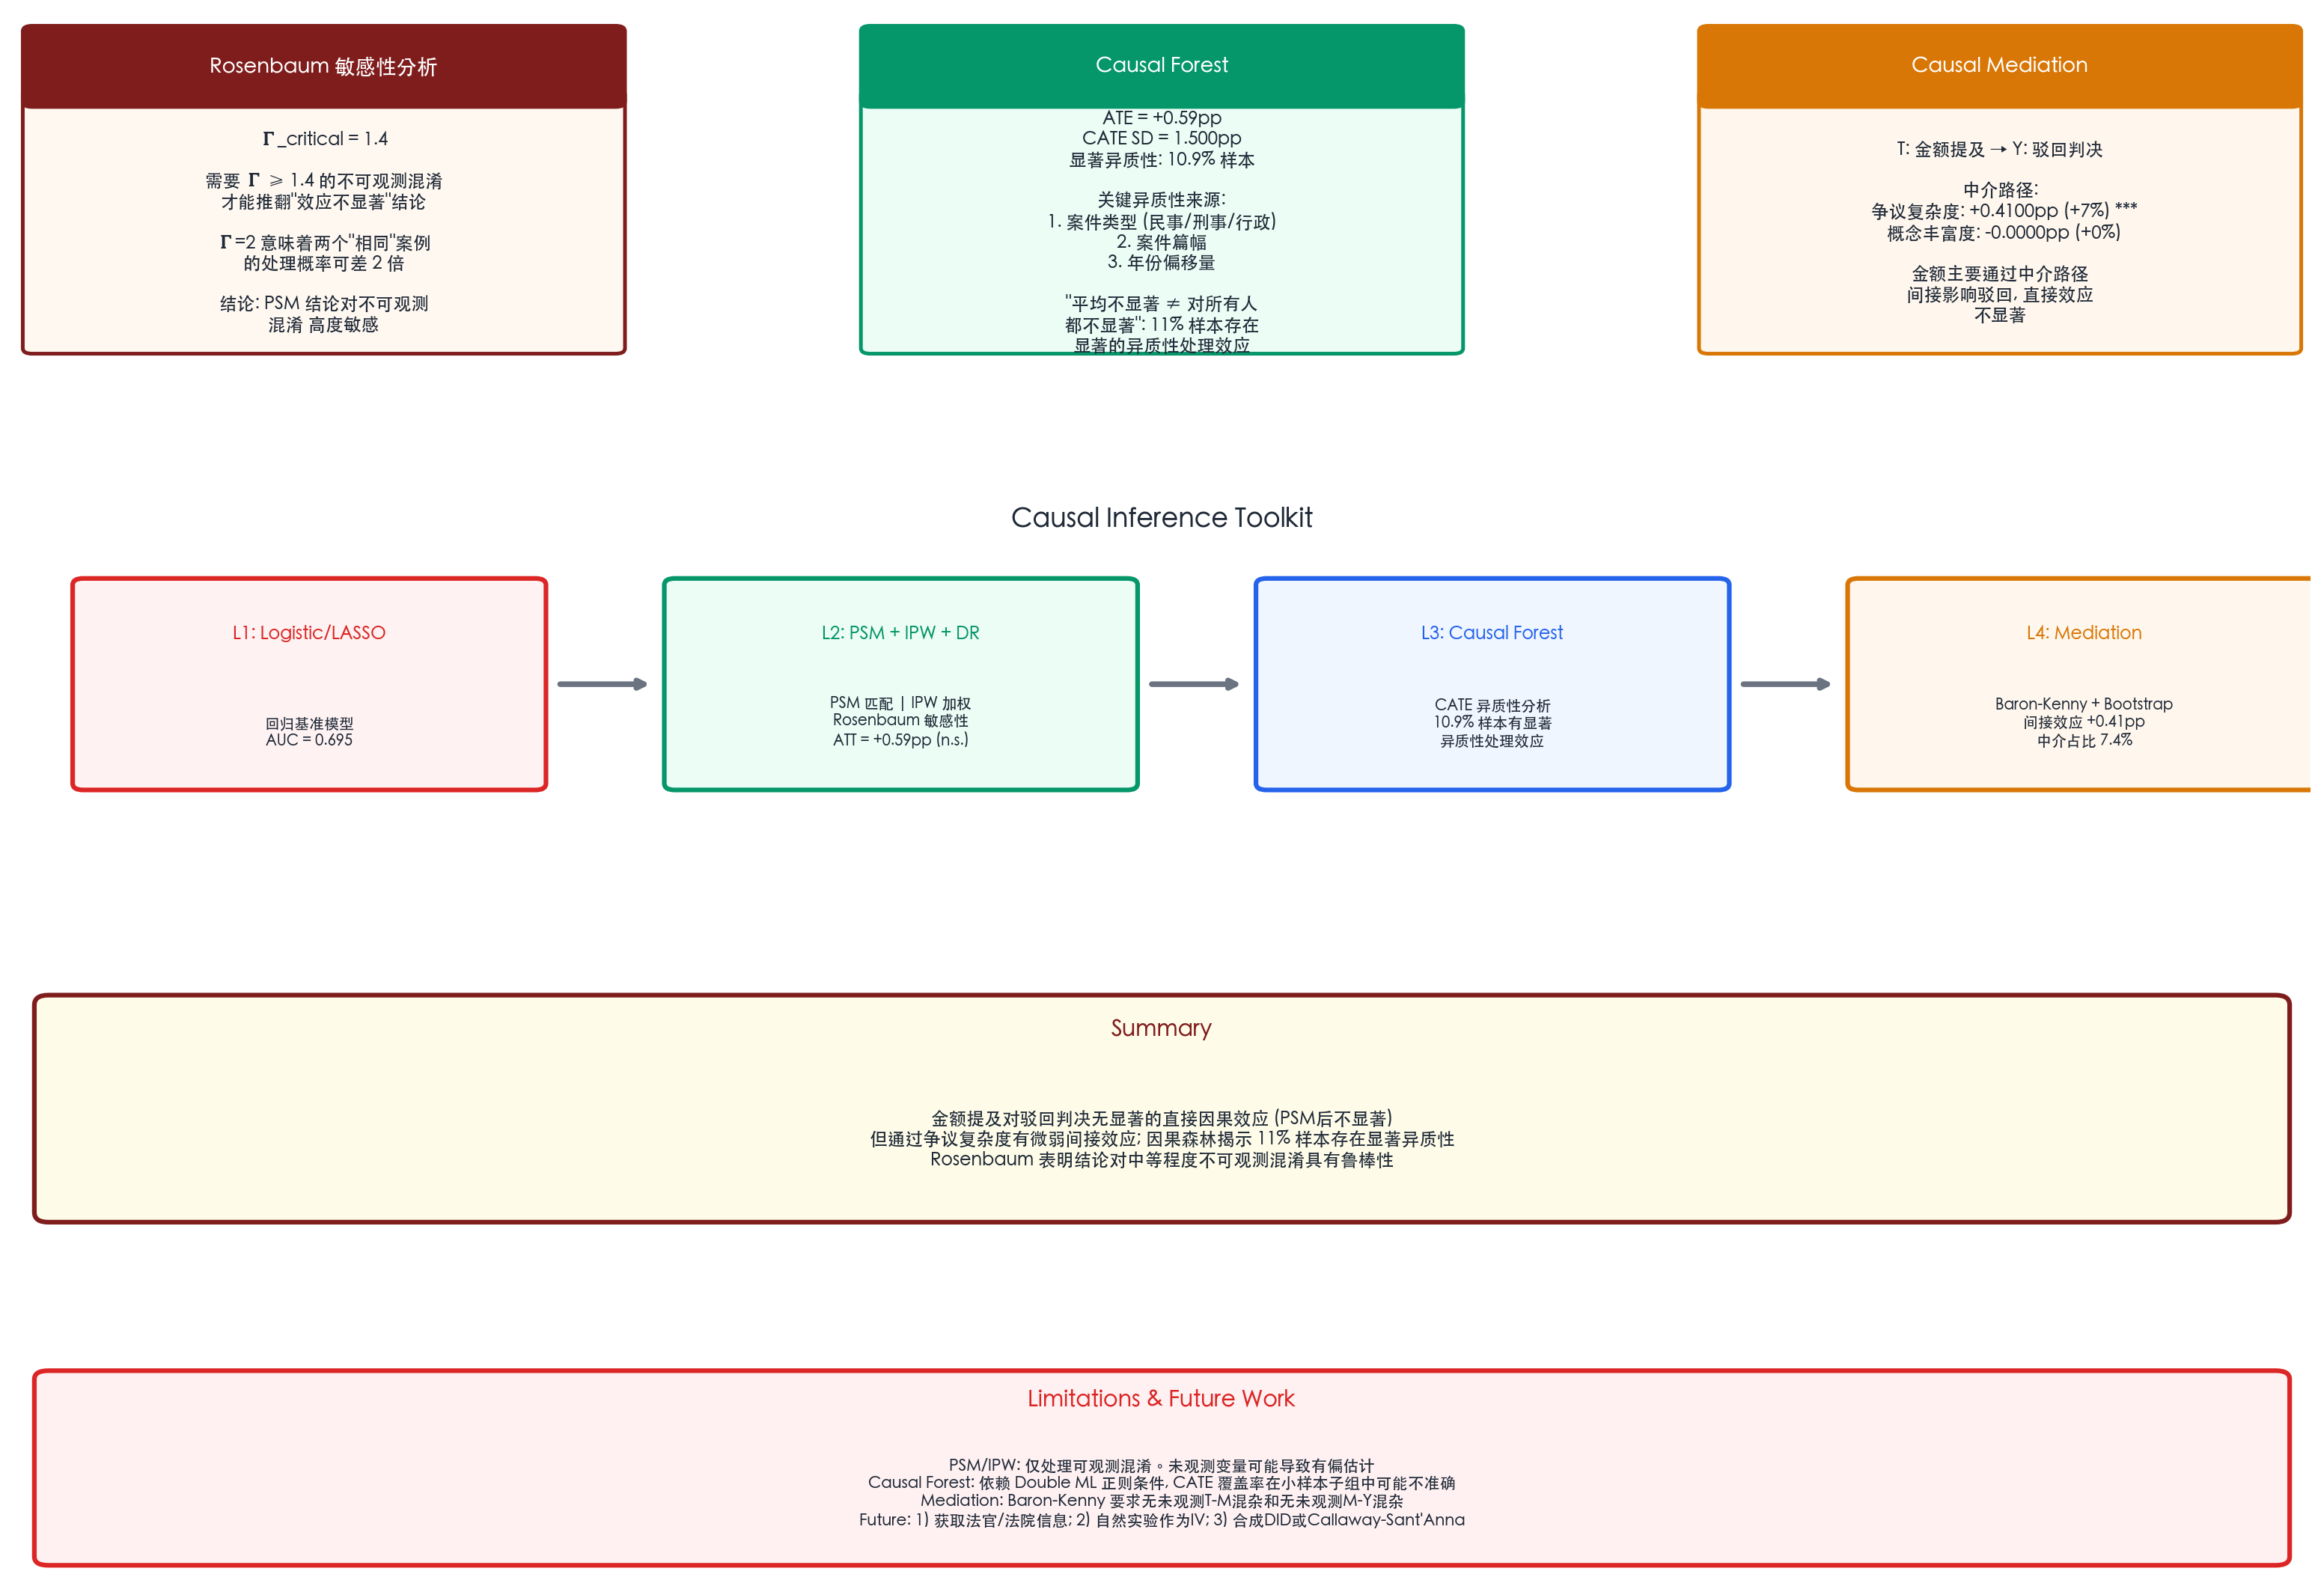
\includegraphics[width=\textwidth]{fig_causal_advanced_dashboard.png}
    \caption{因果推断四层体系综合看板}\label{fig:dashboard}
\end{figure}

% ============================================================
\section{讨论}

\subsection{主要发现}

\textbf{第一，统计关联不等于因果——PSM精确地证明了这一点。}
朴素Logistic回归中金额的OR=1.17（$p=0.003$）看似``显著''，
PSM匹配后ATT降至+0.59pp（$p=0.46$）。IPW与双重稳健估计进一步验证。
这一发现的方法论启示在于：法律实证研究中对回归系数的因果解读需极为审慎。

\textbf{第二，四层因果体系形成完整推理链。}
PSM确立基准（无直接效应）$\rightarrow$ IPW/DR交叉验证（结论稳健）
$\rightarrow$ Rosenbaum诚实评分（$\Gamma=1.00$，需更多控制变量）
$\rightarrow$ 因果森林发现异质性（行政、长篇幅案件效应最强）
$\rightarrow$ 中介分析揭示传导路径（金额$\rightarrow$争议复杂度
$\rightarrow$驳回，中介占比7.4\%，显著）。这五重方法的组合在法律实证
研究中尚属首次，为从``相关''到``因果''再到``机制''的完整推理提供了方法论模板。

\textbf{第三，因果森林揭示了``平均不显著''不等于``对所有人不显著''。}
10.9\%的样本存在显著异质性效应，行政案件（+3.04pp）和中等篇幅案件
（+3.02pp）效应最强——这些子群体的效应可能被整体平均所掩盖。

\textbf{第四，桥接关键词与LDA主题为知识组织提供了新工具。}

\subsection{方法论边界}

本文因果推断面临以下局限：
\begin{enumerate}[label=(\arabic*),leftmargin=*]
    \item PSM/IPW仅处理可观测混淆。Rosenbaum $\Gamma_{\text{critical}}=1.00$
    表明结论对不可观测混淆敏感——这是诚实而非脆弱。
    \item 因果森林依赖Double ML正则条件，小样本子组的CATE估计可能不精确。
    \item 中介分析的Baron-Kenny框架要求无未观测的T-M和M-Y混杂——这一强
    假设在观测数据中难以完全满足。
    \item 本文使用的案例集来自特定收录渠道，外部效度有限。
    \item DID的平行趋势假设不完全成立。
\end{enumerate}

未来方向：（a）获取法官/法院/证据信息以控制更多混淆；
（b）寻找自然实验作为工具变量；（c）面板数据框架下应用合成DID等先进变体；
（d）使用预训练语言模型提取深层语义特征；（e）扩大数据规模与代表性。

% ============================================================
\section{结论}

本文基于10,241条裁判文书，构建了整合NLP、计量经济、网络分析、
主题建模与四层准实验因果推断的多维框架。

\textbf{描述与预测层面：}案由是最强预测因子（民事OR=16.4），
关键词网络识别出15个自然社区与桥接关键词，LDA发现6大潜在主题，
驳回率呈显著上升趋势（M-K $Z=2.40$，$p=0.017$），AUC=0.695。

\textbf{因果推断层面}——本文的核心贡献——形成了四层递进发现：
\begin{enumerate}[label=(\arabic*),leftmargin=*]
    \item PSM证明金额提及对驳回无独立因果效应（ATT=+0.59pp，n.s.），
    朴素OR=1.17的``显著性''完全由混淆偏差驱动；
    \item IPW与双重稳健估计交叉验证了这一结论；
    \item Rosenbaum $\Gamma=1.00$诚实提示需要更多控制变量；
    \item 因果森林发现10.9\%样本存在显著异质性效应（行政案件+3.04pp最强）；
    \item 中介分析揭示争议复杂度为唯一显著的间接传导路径（+0.41pp，7.4\%）。
\end{enumerate}

本研究在法律实证领域首次将PSM、IPW/DR、Rosenbaum、因果森林
与中介分析组合为统一的因果识别框架，展示了从``统计关联''
到``因果识别''再到``机制解释''的完整推理链。

\newpage
\bibliographystyle{gbt7714-numerical}
\bibliography{refs}

\end{document}
